\documentclass[lettersize,journal]{IEEEtran}
\usepackage[T1]{fontenc}
\usepackage{amsmath,amssymb}
\usepackage{booktabs}
\usepackage{multirow}
\usepackage{array}
\usepackage[table]{xcolor}
\usepackage{url}
\usepackage{cite}
\usepackage{tikz}
\usetikzlibrary{positioning,arrows.meta,decorations.pathreplacing,calc,fit}
% Every measured number the paper quotes, in one place. Sources:
%   Jetson: ~/research/measured/<run>/summary.json, pooled over s1-s3
%           (sum tokens / sum time; energy = work-window board DC energy / generated tokens)
%   Pi 5:   ~/Research/measured, pooled over the two subsets with token logs (n=200)
%   gate/diff: benchmark/ae_gate.py
% \pend marks a cell whose run has not finished; nothing in red may be submitted.
\newcommand{\pend}[1]{\textcolor{red}{#1}}

% ---- Jetson Orin Nano 8GB, 15 W, E2B (n=300 each; complete) ----
\newcommand{\EtwoAccL}{52.7}   \newcommand{\EtwoAccG}{53.0}   \newcommand{\EtwoAccA}{53.0}
\newcommand{\EtwoDecL}{23.00}  \newcommand{\EtwoDecG}{25.58}  \newcommand{\EtwoDecA}{29.52}
\newcommand{\EtwoPrmL}{381}    \newcommand{\EtwoPrmG}{1{,}444} \newcommand{\EtwoPrmA}{385}
\newcommand{\EtwoWallL}{31.0}  \newcommand{\EtwoWallG}{28.3}  \newcommand{\EtwoWallA}{24.1}
\newcommand{\EtwoJL}{0.465}    \newcommand{\EtwoJG}{0.446}    \newcommand{\EtwoJA}{0.370}
\newcommand{\EtwoJiL}{0.258}   \newcommand{\EtwoJiG}{0.254}   \newcommand{\EtwoJiA}{0.207}
\newcommand{\EtwoWL}{10.26}    \newcommand{\EtwoWG}{10.86}    \newcommand{\EtwoWA}{10.58}
\newcommand{\EtwoIdent}{300/300}

% ---- Jetson, E4B (complete 2026-10-05) ----
\newcommand{\EfourAccL}{66.0}  \newcommand{\EfourAccG}{65.3}  \newcommand{\EfourAccA}{65.3}
\newcommand{\EfourDecL}{11.62} \newcommand{\EfourDecG}{15.05} \newcommand{\EfourDecA}{17.67}
\newcommand{\EfourPrmL}{381}   \newcommand{\EfourPrmG}{1{,}446} \newcommand{\EfourPrmA}{385}
\newcommand{\EfourWallL}{62.6} \newcommand{\EfourWallG}{51.9} \newcommand{\EfourWallA}{41.6}
\newcommand{\EfourJL}{0.965}   \newcommand{\EfourJG}{0.838}   \newcommand{\EfourJA}{0.676}
\newcommand{\EfourJiL}{0.552}  \newcommand{\EfourJiG}{0.490}  \newcommand{\EfourJiA}{0.396}
\newcommand{\EfourWL}{10.77}   \newcommand{\EfourWG}{11.62}   \newcommand{\EfourWA}{11.39}
\newcommand{\EfourIdent}{300/300}

% ---- headline ratios (S9 vs llama.cpp / vs little-gemma) ----
\newcommand{\EtwoSpL}{1.28}    \newcommand{\EtwoSpG}{1.15}
\newcommand{\EfourSpL}{1.52} \newcommand{\EfourSpG}{1.17}
\newcommand{\EtwoJsav}{20}     \newcommand{\EfourJsav}{30}   % % less J/token than llama.cpp

% ---- Raspberry Pi 5 (llama.cpp, CPU, 3 threads; n=300 accuracy, n=200 rates) ----
\newcommand{\PiEtwoAcc}{51.7}  \newcommand{\PiEtwoDec}{6.87}  \newcommand{\PiEtwoJ}{1.130}  \newcommand{\PiEtwoW}{6.90}
\newcommand{\PiEfourAcc}{65.7} \newcommand{\PiEfourDec}{3.37} \newcommand{\PiEfourJ}{2.223} \newcommand{\PiEfourW}{6.75}

% ---- ablation (mmlupro-ae variants ngram / reuse, s1-s3, n=300; ngram ran 2026-10-05; reuse-only re-run 2026-10-07/08 after the flags bug) ----
% base row = little-gemma (S3): the AE binary with every switch off is byte-identical to it
\newcommand{\AbNgDecEtwo}{29.51} \newcommand{\AbNgPrmEtwo}{1{,}444} \newcommand{\AbNgWallEtwo}{24.8} \newcommand{\AbNgJEtwo}{0.378}
\newcommand{\AbRuDecEtwo}{25.81} \newcommand{\AbRuPrmEtwo}{385} \newcommand{\AbRuWallEtwo}{27.2} \newcommand{\AbRuJEtwo}{0.464$^c$}
\newcommand{\AbNgDecEfour}{17.82} \newcommand{\AbNgPrmEfour}{1{,}444} \newcommand{\AbNgWallEfour}{42.7} \newcommand{\AbNgJEfour}{0.696}
\newcommand{\AbRuDecEfour}{15.47} \newcommand{\AbRuPrmEfour}{385} \newcommand{\AbRuWallEfour}{47.6} \newcommand{\AbRuJEfour}{0.853$^c$}

% ---- where the time goes (pooled n=300, E2B) ----
\newcommand{\PrefShareL}{2.7}   % % of request time in prefill, llama.cpp
\newcommand{\PrefShareG}{3.2}   % little-gemma
\newcommand{\GenTokL}{198{,}706} \newcommand{\GenTokG}{197{,}977}

% ---- iPhone 15 Pro (MLX, GemmaBench; findings/phone, current run per cell; n=300) ----
% decode pooled sum(gt)/sum(gms); energy = whole-phone battery % x capacity estimate / generated tokens
\newcommand{\PhEtwoAcc}{51.0}  \newcommand{\PhEtwoDec}{14.50} \newcommand{\PhEtwoJ}{0.354}
\newcommand{\PhEfourAcc}{66.0} \newcommand{\PhEfourDec}{9.18}  \newcommand{\PhEfourJ}{0.593}

% ---- request-window energy (power integrated over request windows only; J/gen token, pooled s1-s3) ----
\newcommand{\RwEtwoL}{0.458} \newcommand{\RwEtwoG}{0.438} \newcommand{\RwEtwoA}{0.363}
\newcommand{\RwEfourL}{0.948} \newcommand{\RwEfourG}{0.824} \newcommand{\RwEfourA}{0.664}

% ---- llama.cpp + its own n-gram drafting, width 4 (n3m3), n=300, run 2026-10-07/08 ----
\newcommand{\EtwoAccN}{53.3} \newcommand{\EtwoIdN}{29/300$^b$} \newcommand{\EtwoDecN}{26.63} \newcommand{\EtwoPrmN}{381} \newcommand{\EtwoWallN}{27.9} \newcommand{\EtwoWN}{10.84} \newcommand{\EtwoJN}{0.429} \newcommand{\EtwoJiN}{0.228}
\newcommand{\EfourAccN}{65.0} \newcommand{\EfourIdN}{20/300$^b$} \newcommand{\EfourDecN}{13.83} \newcommand{\EfourPrmN}{381} \newcommand{\EfourWallN}{54.3} \newcommand{\EfourWN}{11.53} \newcommand{\EfourJN}{0.871} \newcommand{\EfourJiN}{0.487}


\newcommand{\sys}{CoPR}
\newcommand{\ours}{\sys{}\,(ours)}
\definecolor{oursbg}{gray}{0.88}
\newcolumntype{O}{>{\columncolor{oursbg}}c}
\newcommand{\lc}{llama.cpp}
\newcommand{\lgm}{little-gemma}

\begin{document}

\title{Never Compute Twice: Exact-Output Speedups\\for Gemma~4 on an Edge GPU}

% TODO(author): add \IEEEmembership grades if any, and a funding \thanks if any.
\author{Rifky Ari Yunanto, Jenq-Shiou Leu, and Setya Widyawan Prakosa
\thanks{(Corresponding author: Jenq-Shiou Leu.)}
\thanks{The authors are with the Department of Electronic and Computer
Engineering, National Taiwan University of Science and Technology, Taipei,
Taiwan (e-mail: M11402807@mail.ntust.edu.tw; jsleu@mail.ntust.edu.tw;
d10702804@mail.ntust.edu.tw).}}

\markboth{IEEE Embedded Systems Letters}%
{Yunanto \MakeLowercase{\textit{et al.}}: Never Compute Twice: Exact-Output Speedups for Gemma~4 on an Edge GPU}

\maketitle

\begin{abstract}
Making an embedded language model faster usually changes what it says, which
forces revalidation. We show that on a 15\,W edge GPU, an NVIDIA Jetson Orin Nano
8\,GB, much of that speed can be bought without changing a single output byte.
\sys{} (Context drafting with Prefix Reuse) is a host-side patch to the open
Gemma~4 runtime \lgm{}: it feeds prompt-lookup drafts into \lgm{}'s existing
batched verify and keys its existing prefix snapshot per request, without
touching a kernel. All 2{,}100 \sys{} replies tested, over 500 distinct prompts,
are byte-identical to unmodified \lgm{}'s, while on Gemma~4 E2B and E4B \sys{}
decodes \EtwoSpG$\times$ and \EfourSpG$\times$ faster than \lgm{} and uses
17--19\,\% less board energy per token (\EtwoSpL$\times$, \EfourSpL$\times$
and \EtwoJsav--\EfourJsav\,\% against \lc{}). \lc{}'s own $n$-gram drafting
changed 90--93\,\% of replies at the settings that drafted.
\end{abstract}

\begin{IEEEkeywords}
Edge inference, energy measurement, KV-cache reuse, prompt lookup, speculative decoding
\end{IEEEkeywords}

\section{Introduction}
\IEEEPARstart{O}{n} embedded boards, language-model speed is usually traded for
something: a smaller model, more aggressive quantization, a truncated reasoning
phase. Each changes what the model says, and so must be re-validated on accuracy,
with all the noise a few hundred benchmark questions carry. We ask how much speed
is available \emph{without changing the output at all}, on a Jetson Orin Nano
8\,GB in its 15\,W mode, with Gemma~4~\cite{gemma4} E2B and E4B on
MMLU-Pro~\cite{mmlupro}, comparing the general-purpose runtime \lc{}~\cite{llamacpp}
with \lgm{}~\cite{littlegemma,littlegemmarepo}, a runtime specialized for Gemma~4.

Speculative decoding~\cite{leviathan2023,chen2023} with greedy verification keeps
a drafted token only where it equals the model's own choice, and drafting from the
context itself---prompt-lookup decoding~\cite{pld}, LLMA~\cite{llma},
SuffixDecoding~\cite{suffixdecoding}---needs no draft model, unlike the edge
systems LLMCad~\cite{llmcad} and EdgeLLM~\cite{edgellm}. Prefix
caching~\cite{vllm,sglang} skips known work, but sliding-window layers complicate
it~\cite{vllmhybrid}. We propose no new drafting algorithm. \lgm{} (MIT licence)
already ships a batched verify, built for Gemma~4's draft heads, and a KV snapshot
of a fixed system prompt that copies sliding-window rings whole. We contribute a
144-line host-side patch that feeds context drafts into that verify and keys
that snapshot per request; byte identity as the quality standard; a same-run
comparison of output, speed and board energy; and a model that predicts the
gain from logged replies.

\section{Where the Time Goes}\label{sec:where}
On the E2B baselines, about 97\,\% of request time is decode, and \lgm{} is 11\,\%
faster there (30\,\% on E4B), though it prefills 3.8$\times$ more prompt because it
starts every question from an empty cache. Replies also copy their context: chains
of thought restate options and few-shot phrasing. Because greedy output is
deterministic, a drafter's effect can be computed exactly from recorded replies.
Replaying \lgm{}'s 300 E2B replies with a 3-gram lookup at verify width~3 gives 1.41
tokens per decode step: a match on 47\,\% of steps, with 0.87 tokens accepted per
drafted step.

\section{Design}\label{sec:design}
We build \sys{} as a small modification of the open-source \lgm{}
engine~\cite{littlegemmarepo}, so the \lgm{} and
\sys{} rows run the same program and differ only in three switches.
A small change, applied to both rows, lets the benchmark run: whole rendered
prompts in, replies up to 2{,}048 tokens instead of 1{,}024. The 144 lines of
\sys{} add the switches \texttt{-ngram} (context drafting), \texttt{-reuse}
(prefix reuse) and \texttt{-block}~$B$ (verify width). GPU kernels, sampling and
tokenizer are untouched.

The change is small but the gain is not: \lgm{}'s kernels are already tuned, so
what is left is repeated work---one token per weight pass where the reply
copies its context, and the same few-shot prefix prefilled for every question.
Removing only that makes \lgm{} \EtwoSpG$\times$ and \EfourSpG$\times$ faster
and 17--19\,\% cheaper in energy per token, with identical replies, no
retraining or draft model, and one saved prefix as the only added memory on an
8\,GB board
(Sec.~\ref{sec:results}).

\begin{figure}[t]
\centering
\resizebox{\columnwidth}{!}{%
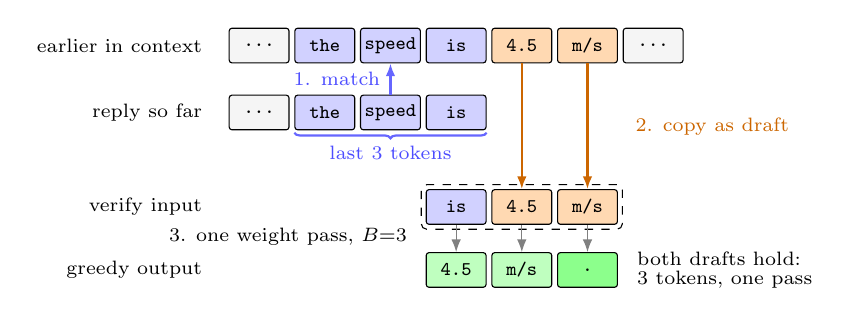
\begin{tikzpicture}[
  tok/.style={draw,rounded corners=1pt,minimum height=4.4mm,minimum width=7.6mm,inner sep=1pt,font=\scriptsize\ttfamily},
  ctx/.style={tok,fill=gray!8},
  key/.style={tok,fill=blue!18},
  cp/.style={tok,fill=orange!30},
  ok/.style={tok,fill=green!25},
  new/.style={tok,fill=green!45},
  lab/.style={font=\scriptsize,anchor=east},
  >={Latex[length=1.6mm]}, node distance=0.6mm]
% row 1: earlier in the context
\node[lab] at (-0.15,0) {earlier in context};
\node[ctx] (a0) at (0.45,0) {...};
\node[key,right=of a0] (a1) {the};
\node[key,right=of a1] (a2) {speed};
\node[key,right=of a2] (a3) {is};
\node[cp,right=of a3]  (a4) {4.5};
\node[cp,right=of a4]  (a5) {m/s};
\node[ctx,right=of a5] (a6) {...};
% row 2: reply so far (its last 3 tokens sit under their earlier match)
\node[lab] at (-0.15,-0.85) {reply so far};
\node[ctx] (b0) at (0.45,-0.85) {...};
\node[key,right=of b0] (b1) {the};
\node[key,right=of b1] (b2) {speed};
\node[key,right=of b2] (b3) {is};
\draw[decorate,decoration={brace,mirror,amplitude=2pt},thick,blue!60]
  ($(b1.south west)+(0,-0.03)$) -- ($(b3.south east)+(0,-0.03)$)
  node[midway,below=1pt,font=\scriptsize,blue!70] {last 3 tokens};
\draw[->,blue!60,thick] (b2.north) -- node[left,font=\scriptsize,blue!70]{1. match} (a2.south);
% row 3: verify (drafts directly under their source)
\node[lab] at (-0.15,-2.05) {verify input};
\node[key] (v0) at (a3 |- 0,-2.05) {is};
\node[cp]  (v1) at (a4 |- 0,-2.05) {4.5};
\node[cp]  (v2) at (a5 |- 0,-2.05) {m/s};
\draw[->,orange!80!black,thick] (a4.south) -- (v1.north);
\draw[->,orange!80!black,thick] (a5.south) -- (v2.north);
\node[font=\scriptsize,orange!80!black,anchor=west] at ($(a5.south east)!0.5!(v2.north east)+(0.1,0)$) {2. copy as draft};
\node[draw,dashed,rounded corners=2pt,fit=(v0)(v2),inner sep=1.6pt] (vb) {};
\node[font=\scriptsize,anchor=east] at ($(vb.west)+(-0.05,-0.38)$) {3. one weight pass, $B{=}3$};
% row 4: greedy outputs
\node[lab] at (-0.15,-2.85) {greedy output};
\node[ok]  (o0) at (v0 |- 0,-2.85) {4.5};
\node[ok]  (o1) at (v1 |- 0,-2.85) {m/s};
\node[new] (o2) at (v2 |- 0,-2.85) {.};
\foreach \i in {0,1,2} \draw[->,gray] (v\i.south) -- (o\i.north);
\node[font=\scriptsize,anchor=west,align=left] at ($(o2.east)+(0.12,0)$)
  {both drafts hold:\\[-1pt]3 tokens, one pass};
\end{tikzpicture}}
\caption{Prompt-lookup drafting with greedy verification. (1) The last three
tokens of the reply are matched against their most recent earlier occurrence in
prompt or reply. (2) The tokens that followed it become the draft. (3) One
batched forward pass computes the model's own greedy choice after every input
position. Drafts are accepted left to right while they equal those choices; the
first mismatch is replaced by the model's choice and the rest discarded, so the
emitted text is exactly what one-token-at-a-time greedy decoding produces. Here
both drafts hold and the pass also yields the next token.}
\label{fig:lookup}
\end{figure}

\textbf{Prompt-lookup drafting} (Fig.~\ref{fig:lookup}). At each step the engine
searches backwards for the most recent earlier occurrence of the last three tokens,
falling back to two, and proposes the up to $B{-}1$ tokens that followed it.
\lgm{}'s batched verify computes every position's
greedy successor in one weight pass and accepts the longest matching prefix. Every step yields one token; if a fraction $m$ of steps draft, each accepting
on average $a$ drafted tokens on top of it, and a drafted step costs $c$ plain
steps, decode speeds up by
\begin{equation}\label{eq:speedup}
S = (1 + m\,a)\,/\,(1 + m\,(c - 1)) .
\end{equation}

\begin{figure}[t]
\centering
\resizebox{\columnwidth}{!}{%
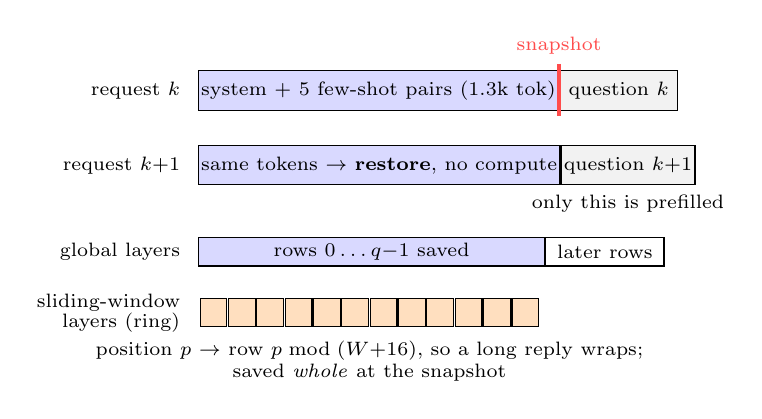
\begin{tikzpicture}[
  seg/.style={draw,minimum height=5mm,inner sep=1pt,font=\scriptsize},
  lab/.style={font=\scriptsize,anchor=east},
  >={Latex[length=1.6mm]}]
% request k
\node[lab] at (-0.1,0) {request $k$};
\node[seg,fill=blue!15,minimum width=4.4cm,anchor=west] (pk) at (0,0) {system + 5 few-shot pairs (1.3k tok)};
\node[seg,fill=gray!10,minimum width=1.5cm,anchor=west] (qk) at (pk.east) {question $k$};
\draw[very thick,red!70] (pk.north east) ++(0,0.08) -- ++(0,-0.66);
\node[font=\scriptsize,red!70,anchor=south] at ($(pk.north east)+(0,0.08)$) {snapshot};
% request k+1
\node[lab] at (-0.1,-0.95) {request $k{+}1$};
\node[seg,fill=blue!15,minimum width=4.4cm,anchor=west] (pk1) at (0,-0.95) {same tokens $\to$ \textbf{restore}, no compute};
\node[seg,fill=gray!10,minimum width=1.5cm,anchor=west] (qk1) at (pk1.east) {question $k{+}1$};
\node[font=\scriptsize,anchor=north] at (qk1.south) {only this is prefilled};
% KV layout
\node[lab] at (-0.1,-2.05) {global layers};
\node[seg,fill=blue!15,minimum width=4.4cm,anchor=west,minimum height=3.6mm] (g) at (0,-2.05) {rows $0\ldots q{-}1$ saved};
\node[seg,fill=white,minimum width=1.5cm,anchor=west,minimum height=3.6mm] at (g.east) {later rows};
\node[lab] at (-0.1,-2.7) {sliding-window};
\node[lab] at (-0.1,-2.95) {layers (ring)};
\foreach \i in {0,...,11} {
  \node[draw,minimum width=3.4mm,minimum height=3.6mm,inner sep=0pt,fill=orange!25] (r\i) at (0.2+\i*0.36,-2.82) {};
}
\node[font=\scriptsize,anchor=north,align=center] at ($(r5.south)+(0.18,-0.05)$) {position $p$ $\to$ row $p \bmod (W{+}16)$, so a long reply wraps;\\saved \emph{whole} at the snapshot};
\end{tikzpicture}}
\caption{Shared-prefix KV reuse. A request that misses the cached prefix saves
the KV state at the start of its final user turn; the next request whose
prompt begins with exactly those tokens restores it and prefills only its
question. Global-attention rows below the snapshot are never overwritten by
later positions of the same subject, but the sliding-window layers are rings
that a long reply wraps over, so the ring is stored whole---its exact content
at the snapshot position---and rewritten on restore.}
\label{fig:reuse}
\end{figure}

\textbf{Shared-prefix KV reuse} (Fig.~\ref{fig:reuse}). Prompts for one subject differ only in the final
user turn. On a miss, \sys{} prefills to the start of that turn, saves the KV state
with \lgm{}'s own save routine, and continues; the next request beginning with
exactly those tokens restores it and prefills only its question. That routine
already copies each sliding-window ring whole, so the snapshot is exact although
rings wrap during a long reply. \sys{} allocates its buffers once instead of per
save (39\,MiB on E2B, 114\,MiB on E4B). With one snapshot, reuse relies on
lm-eval sending a subject's questions together: it restores on 85--86 of every
100 requests, missing once per subject change.

\textbf{Exactness.} The output equals plain greedy decoding only if (i) the batched
verify yields logits bit-identical to a single-token step, and (ii) prefilling two
spans writes the same KV rows as prefilling one. Neither holds in general, so we
treat exactness as an empirical property and compare every reply byte for byte
with unmodified \lgm{}'s; we did not compare logits.

\section{Methodology}\label{sec:method}
All engines load the same QAT \texttt{UD-Q4\_K\_XL} GGUF and run 3 disjoint
stratified subsets of 100 questions ($n{=}300$), 5-shot chain of thought via
lm-eval~\cite{lmeval}, greedy, with a 2{,}048-token answer cap, 8{,}192 context and
thinking off, at GPU 612\,MHz and CPU 1{,}497.6\,MHz caps. \sys{} is \lgm{} with
\texttt{-reuse -ngram -block 3}. Byte
identity is a sharp test: replies average 660 tokens, so one flipped greedy
choice shows, and \lc{}'s own drafting altered 90--93\,\% of its replies. Energy
integrates the INA3221 \texttt{VDD\_IN} rail at 1\,Hz over the working window; it is
board DC input, not wall power. One batch---\lc{}'s $n$-gram drafting, the
reuse-only ablation and a \sys{} repeat---ran with the CPU clock pinned. That
raises energy, so we report only speed for it, and an \lc{} rerun that never
drafted came out 3.3\,\% faster than its unpinned twin, so speed differences
under 3\,\% against those runs are not attributed to the engine. Each
configuration ran once per subset; decode rates vary at most 2.2\,\% between
subsets, and every speedup holds on each subset. An earlier clock fault was
caught before any reported run.

\begin{table*}[t]
\caption{Engines on the Jetson Orin Nano 8\,GB at 15\,W, MMLU-Pro, $n{=}300$ per cell.
Energy is board DC energy over the working window per generated token. \textbf{Bold}: best in row, whichever engine; shaded: the
proposed system. The \lc{} column runs without speculative decoding;
\lc{}+$n$-gram is \lc{}'s own drafting at the fastest of the three settings
tried (width~4, not exact); its power and energy are not reported (--,
Sec.~\ref{sec:method}). Lowest power is not bolded: it does not imply lowest
energy.}
\label{tab:main}
\centering
\setlength{\tabcolsep}{3.8pt}
\begin{tabular}{@{}l cccO cccO@{}}
\toprule
& \multicolumn{4}{c}{Gemma~4 E2B} & \multicolumn{4}{c}{Gemma~4 E4B} \\
\cmidrule(lr){2-5}\cmidrule(lr){6-9}
& \lc{} & \lc{}+$n$-gram & \lgm{} & \ours & \lc{} & \lc{}+$n$-gram & \lgm{} & \ours \\
\midrule
Accuracy (\%)$^a$              & \EtwoAccL & \EtwoAccN & \EtwoAccG & \EtwoAccA & \EfourAccL & \EfourAccN & \EfourAccG & \EfourAccA \\
Identical to \lgm{}$^b$         & 32/300 & 34/300 & ref. & \textbf{\EtwoIdent} & 28/300 & 20/300 & ref. & \textbf{\EfourIdent} \\
Exact: identical without drafting$^c$ & ref. & 29/300 & ref. & \textbf{\EtwoIdent} & ref. & 20/300 & ref. & \textbf{\EfourIdent} \\
Decode (tok/s)                 & \EtwoDecL & \EtwoDecN & \EtwoDecG & \textbf{\EtwoDecA} & \EfourDecL & \EfourDecN & \EfourDecG & \textbf{\EfourDecA} \\
Prompt tokens processed / q    & \textbf{\EtwoPrmL} & \textbf{\EtwoPrmN} & \EtwoPrmG & \EtwoPrmA & \textbf{\EfourPrmL} & \textbf{\EfourPrmN} & \EfourPrmG$^d$ & \EfourPrmA \\
Wall time / question (s)       & \EtwoWallL & \EtwoWallN & \EtwoWallG & \textbf{\EtwoWallA} & \EfourWallL & \EfourWallN & \EfourWallG$^d$ & \textbf{\EfourWallA} \\
Mean power, generating (W)     & \EtwoWL & -- & \EtwoWG & \EtwoWA & \EfourWL & -- & \EfourWG & \EfourWA \\
Energy / gen.\ token (J)       & \EtwoJL & -- & \EtwoJG & \textbf{\EtwoJA} & \EfourJL & -- & \EfourJG & \textbf{\EfourJA} \\
\quad above idle (J)           & \EtwoJiL & -- & \EtwoJiG & \textbf{\EtwoJiA} & \EfourJiL & -- & \EfourJiG & \textbf{\EfourJiA} \\
\bottomrule
\multicolumn{9}{@{}l}{\footnotesize $^a$ Not bolded: all engines are statistically tied (Sec.~\ref{sec:results}).}\\
\multicolumn{9}{@{}l}{\footnotesize $^b$ Byte-identical to \lgm{}'s replies, same 300 questions; ref.: the reference itself.}\\
\multicolumn{9}{@{}l}{\footnotesize $^c$ Byte-identical to the same engine without drafting (\sys{}: to \lgm{}); the exactness test.}\\
\multicolumn{9}{@{}l}{\footnotesize $^d$ One subset re-sent 5 prompts (105 requests); figures divide by its 100 questions, so they include the re-sends.}
\end{tabular}
\end{table*}

\section{Results}\label{sec:results}
\textbf{Quality.} \sys{} reproduces all 300 of \lgm{}'s replies on each model
(Table~\ref{tab:main}), as do the 1{,}200 replies of the ablation runs, the 100 of a
repeat, and the 200 tool calls below: 2{,}100 of 2{,}100, over 500 distinct
prompts. Accuracy is therefore \lgm{}'s: 53.0\,\% on E2B, tied with \lc{}'s
52.7\,\% (exact McNemar $p{=}1.00$), and 65.3\,\% on E4B against \lc{}'s
66.0\,\%.

\textbf{Speed and energy.} \sys{} decodes \EtwoSpG$\times$ faster than the \lgm{}
it patches on E2B and \EfourSpG$\times$ on E4B (per subset 1.148--1.158$\times$ and
1.160--1.189$\times$). Against \lc{} the factors are \EtwoSpL$\times$ and
\EfourSpL$\times$, of which \lgm{}'s own engine advantage is 1.11$\times$ and
1.30$\times$. Reuse brings prompt tokens processed from \EtwoPrmG{} per question to
\EtwoPrmA{}, level with \lc{}. Wall time per question falls 15\,\% and 20\,\%
against \lgm{} (22\,\% and 34\,\% against \lc{}). Power barely moves
(10.3--11.6\,W), so energy per token follows time: 17\,\% and 19\,\% below \lgm{},
\EtwoJsav\,\% and \EfourJsav\,\% below \lc{}.

\begin{table}[t]
\caption{\lc{}'s own $n$-gram drafting against \sys{}, E2B, subset s1 ($n{=}100$). ``Exact'': replies identical to the
same engine without drafting (ref.: that engine itself; for \sys{}, \lgm{}).
Bold: best per column; accuracy not bolded (all tied).}
\label{tab:lcngram}
\centering\footnotesize
\setlength{\tabcolsep}{4pt}
\begin{tabular}{@{}lcccc@{}}
\toprule
& Exact & Acc. & Decode & Wall \\
& & (\%) & (tok/s) & (s/q) \\
\midrule
\lc{}, no drafting & ref.    & 56 & 23.04 & 27.9 \\
\lc{} $n$-gram, width 3$^\S$ & n/a & 56 & 23.80 & 27.4 \\
\lc{} $n$-gram, width 4 & 8/100   & 56 & 26.97 & 26.1 \\
\lc{} $n$-gram, stock & 9/100   & 53 & 25.15 & 26.8 \\
\rowcolor{oursbg}\ours, width 3 & \textbf{100/100} & 54 & \textbf{29.54} & \textbf{23.8} \\
\bottomrule
\multicolumn{5}{@{}l}{\footnotesize $^\S$ Never drafted (no draft logged in any request): a plain}\\
\multicolumn{5}{@{}l}{\footnotesize \phantom{$^\S$} rerun, so exactness is not applicable (n/a).}\\
\end{tabular}
\end{table}

\textbf{Against \lc{}'s $n$-gram drafting} (Table~\ref{tab:lcngram}). At the
fastest of three settings tried (\texttt{-{}-spec-type ngram-simple}, width~4),
\lc{} changes 271 of 300 E2B and 280 of 300 E4B replies relative to its own
plain decoding, with accuracy tied (McNemar $p{=}0.86$ and $0.69$). The likely
mechanism is that GPU matrix kernels use different tilings and reduction orders
for one token and for several, breaking condition~(i); we did not isolate the
kernel. \sys{} still decodes 1.11$\times$ and 1.28$\times$ faster and answers
questions 14\,\% and 23\,\% sooner.

\begin{table}[t]
\caption{Ablation, $n{=}300$ per row. The first row is \lgm{}; \sys{} with
every switch off reproduced it byte for byte on two pre-run gate checks of 14
and 28 questions (a 300-question no-switch run was not made). Every other row's
replies are byte-identical to \lgm{}'s (1{,}800 replies). The reuse-only rows
ran with pinned clocks. Bold: best per column within a model.}
\label{tab:ablation}
\centering\footnotesize
\setlength{\tabcolsep}{3pt}
\begin{tabular}{@{}l cccc@{}}
\toprule
& Decode & Prompt & Wall & J / \\
& (tok/s) & tok / q & s / q & tok \\
\midrule
\multicolumn{5}{@{}l}{\emph{Gemma~4 E2B}} \\
\lgm{} (no switches)   & \EtwoDecG & \EtwoPrmG & \EtwoWallG & \EtwoJG \\
+ prompt lookup        & \AbNgDecEtwo & \AbNgPrmEtwo & \AbNgWallEtwo & \AbNgJEtwo \\
+ prefix reuse         & \AbRuDecEtwo & \textbf{\AbRuPrmEtwo} & \AbRuWallEtwo & \AbRuJEtwo \\
\rowcolor{oursbg}+ both (\ours)        & \textbf{\EtwoDecA} & \textbf{\EtwoPrmA} & \textbf{\EtwoWallA} & \textbf{\EtwoJA} \\
\midrule
\multicolumn{5}{@{}l}{\emph{Gemma~4 E4B}} \\
\lgm{} (no switches)   & \EfourDecG & \EfourPrmG & \EfourWallG & \EfourJG \\
+ prompt lookup        & \textbf{\AbNgDecEfour} & \AbNgPrmEfour & \AbNgWallEfour & \AbNgJEfour \\
+ prefix reuse         & \AbRuDecEfour & \textbf{\AbRuPrmEfour} & \AbRuWallEfour & \AbRuJEfour \\
\rowcolor{oursbg}+ both (\ours)        & \EfourDecA & \textbf{\EfourPrmA} & \textbf{\EfourWallA} & \textbf{\EfourJA} \\
\bottomrule
\multicolumn{5}{@{}l}{\footnotesize $^a$ Not reported: run with pinned clocks (Sec.~\ref{sec:method}).}
\end{tabular}
\end{table}

\textbf{Ablation} (Table~\ref{tab:ablation}). Prompt lookup alone delivers nearly all of the decode gain (29.51
against 29.52\,tok/s on E2B, 17.82 against 17.67 on E4B) and $-$15\,\% and $-$17\,\%
energy per token against \lgm{}. Reuse alone cuts prompt tokens processed by
73\,\%; its $+$1--3\,\% decode is within the pinned-clock bound.

\textbf{Verify width and overhead.} On E2B, a drafted step at widths 2, 3 and 4
accepts 0.57, 0.90 and 1.12 tokens and costs 1.24, 1.47 and 1.76 plain decode steps.
Width~3 was fastest on both models (E2B: 29.62, 29.93 and 28.81\,tok/s at widths
2--4, against 25.63 without drafting), by only 1.0\,\% and 0.8\,\% over width~2 in a
28-question sweep, so we take it as a reasonable default, not a proven optimum. The
accepted counts match the offline replay (0.55, 0.87, 1.08) within 0.04 tokens,
and Eq.~\eqref{eq:speedup} with the replayed $m$, $a$ and the measured $c$
predicts 1.14, 1.15 and 1.11$\times$ against 1.16, 1.17 and 1.12$\times$
measured, picking the same width before any engine change. A worst-case lookup
took 68\,$\mu$s against about 39\,ms for a decode step.

\textbf{Tool calls and instructions.} On 200 BFCL~\cite{bfcl}
prompts, all \sys{} calls equal \lgm{}'s; replay gives 1.24 tokens per decode
step, and live decode rises 12\,\% (each request 6\,\% sooner). Replay on 100
IFEval~\cite{ifeval} replies, not run live, gives only 1.10, a predicted
$\approx$2\,\% gain. Prefix reuse never fired on BFCL, because per-request tool
schemas precede the final user turn.

\section{Limitations and Conclusion}\label{sec:limits}
The engine comparison covers one board in its 15\,W mode and greedy decoding,
with tool calls on E2B only; under sampling, acceptance falls. Drafting with
Gemma~4's trained draft heads is out of scope. \sys{} inherits \lgm{}'s scope, the Gemma~4 family on CUDA. Within that
scope, two host-side changes to \lgm{} make it decode \EtwoSpG$\times$ and
\EfourSpG$\times$ faster without changing one byte of its answers, and the gain
follows how much a workload copies its context. Both changes to \lgm{}, scripts, logs, all
replies including failed runs, and a script that recomputes the tables are at
\url{https://github.com/rifkyariy/agentic-edge}.

\bibliographystyle{IEEEtran}
\bibliography{refs}

\end{document}
